%!TEX root = D2.1_AMIDSTModellingFramework.tex
\subsection{CajaMar Models}
\label{Section:CajaMarModels}

\subsubsection{Introduction}

There are two tasks to be solved for Cajamar's use case (see D1.2 and DoW). The main one is
the estimation of the \emph{probability of default}, defined as the probability that a
credit operation will end up in default within two years. The secondary task consists in obtaining 
good customer profiles in terms of risk, so that marketing campaigns can be
specifically targeted to these low risk customers. 

%%%%%%%%%%%%%%%%%%%%%%%%%%%%%%%%%%%%
\subsubsection{Predicting probability of default}
\label{SubSection:Predicting}
%%%%%%%%%%%%%%%%%%%%%%%%%%%%%%%%%%%%

%---------------------------------------------------------------------------------------------
\subsubsection*{Introduction of the problem} 

In any commercial bank, every time a customer applies for a loan, the bank experts evaluate the customer's risk profile before making their decision. 

At Cajamar, this risk evaluation protocol is implemented by evaluating whether the client is going to default or not within the following two years. At the moment of writing, this decision is supported by an automatic supervised classification model (i.e. a logistic regression) which takes information about the recent financial activity of the customer at CajaMar, as well as information about the recent past paying behaviour of the customer provided by other Spanish financial institutions, and make predictions using this information about the probability that the client will default during the following two years.

The methodology currently employed does not assume dependence structure among the variables. Even though this model is quite simple, current predictions are made using only a set of $27$ variables out of the more than $1000$ that are available. Updates in risk predictions are made on a monthly basis, whereas the predictive model is only updated after several years. These low update frequencies are selected partly due to limitations in the available commercial software and the computing resources.

The objective is to daily update the risk evaluation for every customer of the bank. This daily evaluation will be made by creating two data sets: the model training data set and the model evaluation data set (see Use Case 1 in D1.2). How these data sets are created gives us some insights about the nature of this risk prediction problem.  Figure \ref{Figure:CajaMarTimeLine} shows the time-line of the generation of the evaluation and training data set, which is further explained below. 


\begin{figure}
\begin{center}
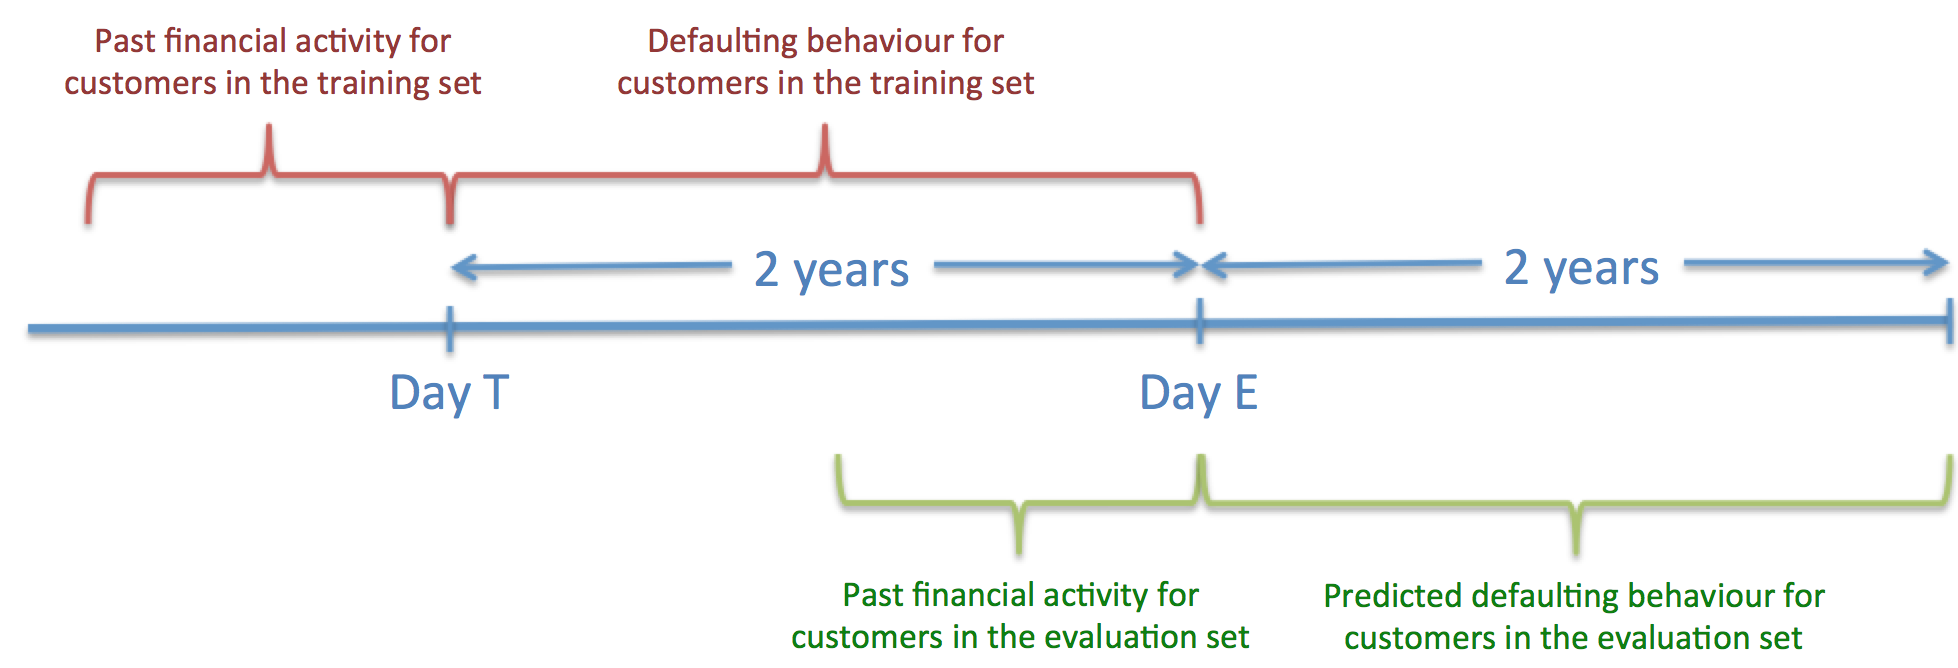
\includegraphics[scale=0.4]{figures/CajarMarTimeLine}
\caption{\label{Figure:CajaMarTimeLine}Time-line of the generation of the evaluation and training data sets.}
\end{center}
\end{figure}

\begin{itemize}
\item \textbf{Model Evaluation Data Set:} We denote by day $E$ to the day at which this evaluation data set is created. This data set contains a record for every client to be evaluated at that day $E$. As in any standard evaluation data set in supervised classification settings, each record will contain the values of the predictors variables for this customer. The predictor variables refers to the financial activity and the paying behaviour of the customers in a recent past and their socio-demographics data. 

The recent financial activity refers to attributes of the customer such as ``account balance'', ``number of credit card operations'', etc. in the last 180 days \footnote{This limit is fixed by the Bank of Spain}. These attributes usually change daily for a customer, then they are encoded by introducing a set of variables for each attribute that contains the value of this attribute in the last 180 days from day $E$. I.e. if the financial activity of the customer is detailed by $F$ attributes,   $180\cdot F$ predictive variables are included in this data set.

In the case of past paying behaviour, the attributes refers to attributes such as the paying behaviour of the customer with other financial institutions or other companies (phone companies, electricity companies, public bodies, etc.). A monthly record of the last 36 months from day $T$ is considered when building the evaluation data set. So, if there are $P$ variables referring to the paying behaviour of a customer, $36\cdot P$ variables are included as information about the past paying behaviour.  

The task of the supervised classification model is to take each of the records (i.e. customers) of this data set and compute the probability of defaulting within the following two years. If at some point the probability of defaulting of some customers rises above some predefined threshold, the bank can try to take preventive actions to reduce the chances that this customer finally defaults in some of his/her loans.

\item \textbf{Model Training Data Set:}  The training data set is built in the same way than the evaluation data set. They contain the same set of predictive variables with the main difference that they refer to different time points. If the predictive variables in the evaluation data set are built for day $E$, the predictive variables in the training data set are defined for the day $T = E$ - 2 years (i.e. two years before in time). So the training data set contain one record for each customer of the bank and the predictive variables refers to the financial activity and paying behaviour of this customer in the recent past before day $T$ (i.e. the previous 180 days or the previous 36 months). 

Unlike the evaluation data set, each record of this data set contains a class label indicating if this customer is defaulter o non-defaulter. To decide if a customer is defaulter or not, we look at the 2 years data between day $T$ and current day $E$. If during these two years the client has regularly pay each of his/her loans and the other financial institutions does not provide any evidence of defaulting, the client is labelled as non-defaulter. Otherwise, it is labelled as defaulter (see Data Characteristics document for more detailed information about this respect).   

Using this data set, the bank fits a logistic regression model, which is then used to update the probability of defaulting of each of the clients in the evaluation data set. 

\end{itemize}




\subsubsection*{Static Model} 

In this first approach we do not explicitly consider some of the dynamics of the problem: we do not model that a customer can be non-defaulter and defaulter at different moments in time (e.g. one customer can be creditworthy and, after some time, go bankrupt due to unemployment). Instead, we consider a static prediction model where given the financial behaviour of the client over a recent past, it predicts whether the client will default or not within the next 2 years. Similarly to what it is done in the current CajaMar approach. 

Figure \ref{Figure:CajaMarStatic} shows the general structure of this static model. Each yellow box represents a set of $F$ variable measurements for a particular day.
For the shake of simplicity, for now on and in the graphical models depicted, we do not explicitly show the variables that refer to monthly information during the last 36 months. The green node is the class variable that represents the probability that a customer will default within the next two years. 

\begin{figure}
\begin{center}
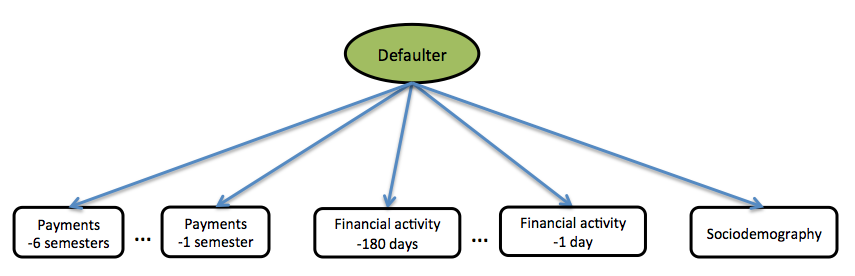
\includegraphics[scale=0.45]{./figures/CajaMarModel0}
\caption{\label{Figure:CajaMarStatic}Global structure of the static model. Each blue box represents a set of variables measures during the same day.
The variables within a box can be connected (e.g. according to a tree structure and, globally, conforming a TAN).}
\label{fig:static}
\end{center}
\end{figure}

The variables within a box can be connected (e.g. according to a tree structure and, globally, conforming a TAN). \textcolor{blue}{Figure \ref{Figure:cajamarDependences}(a) shows how indeed there exist dependences between some of the variables in the data for a particular day. \textcolor{red}{Please replace this BN by another one with the name of some of the variables}. Figure \ref{Figure:cajamarDependences}(b) shows the contour bivariate plot for variables V1 and V2, showing a clear linear relationship between the two variables. This might even indicate that one variable is just a replica of the other variable or contain quite similar information, and their joint contribution will not only make learning and inference computationally more expensive, but it could lead to poorer performance []. This would contribute to support the need to explore suitable feature selection techniques as specified in Use Case 2 of Cajamar's Requirement analysis.}

\begin{figure}
  \centering
    \begin{tabular}{cc}
    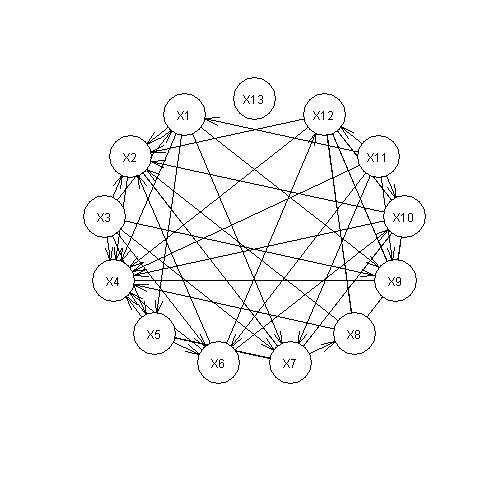
\includegraphics[width=70mm]{figures/CajaMarBayesianNetwork}&
    \begin{minipage}[b]{0.45\linewidth} Contour plot to be included with (ideally) strong linear correlation between variables (maybe class-conditioned?) \end{minipage}\\
  \end{tabular}
    \caption{\label{Figure:cajamarDependences}.}
\end{figure}

It is also of major interest to analyse the type of density probability distributions to use in the proposed model. Figures \ref{Figure:cajamarMixt}(a) and (b) show the density histogram for the values of a continuos attribute that measures the end-of-day balance for defaulters and non-defaulters respectively. The density curves represent a credible approximation using mixture of Gaussian distributions, which is the case for most of the other predictive attributes. Note that for defaulters, the values of the end-of-day balance are overall lower compared to those corresponding to non-defaulters.

\begin{figure}
  \centering
    \begin{tabular}{cc}
    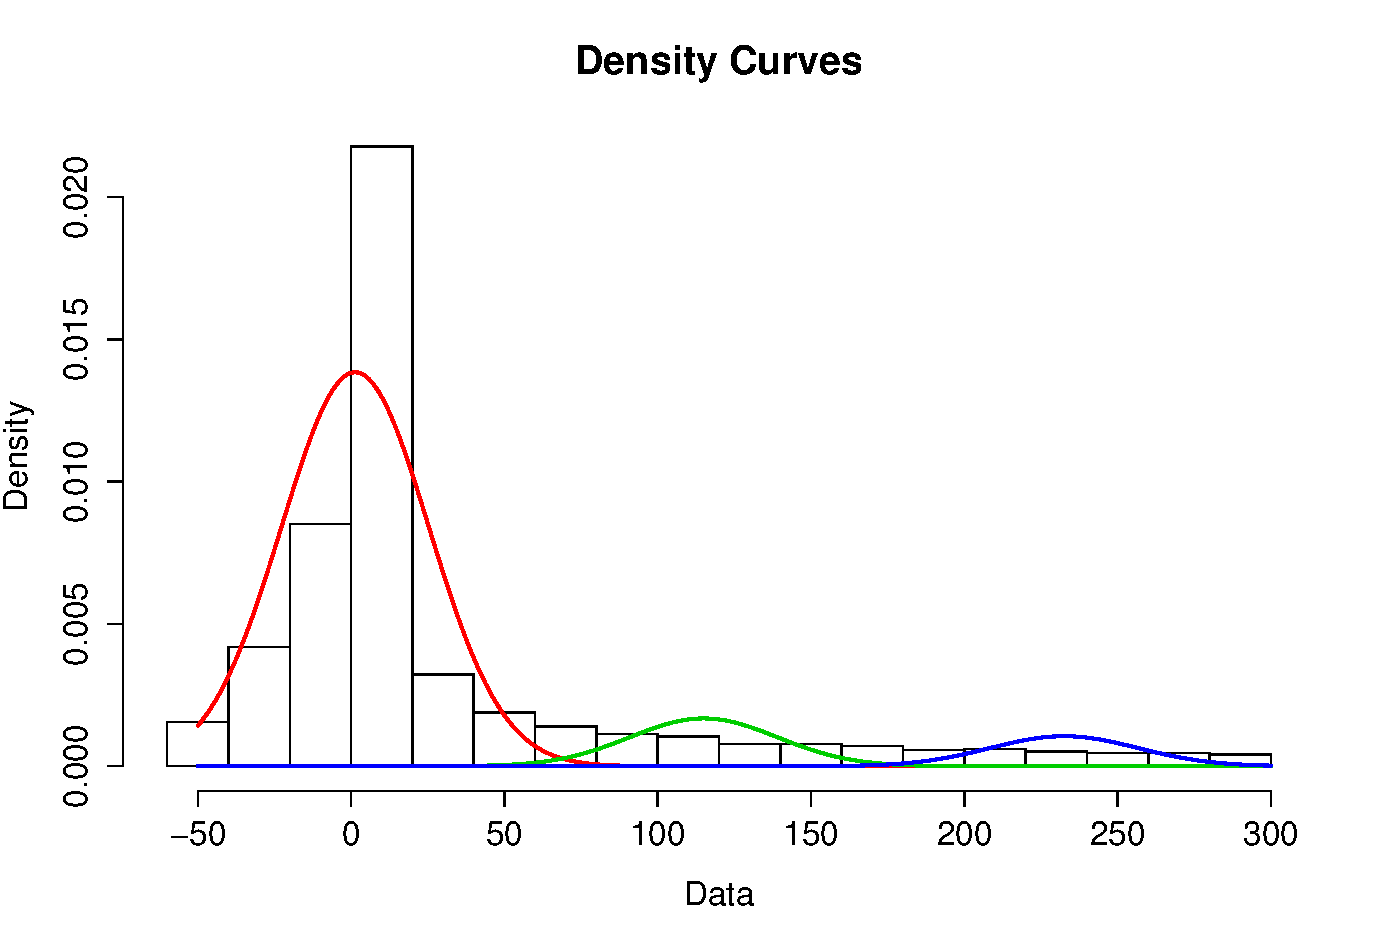
\includegraphics[width=70mm]{figures/CajaMarmixtureBalanceDef}&
    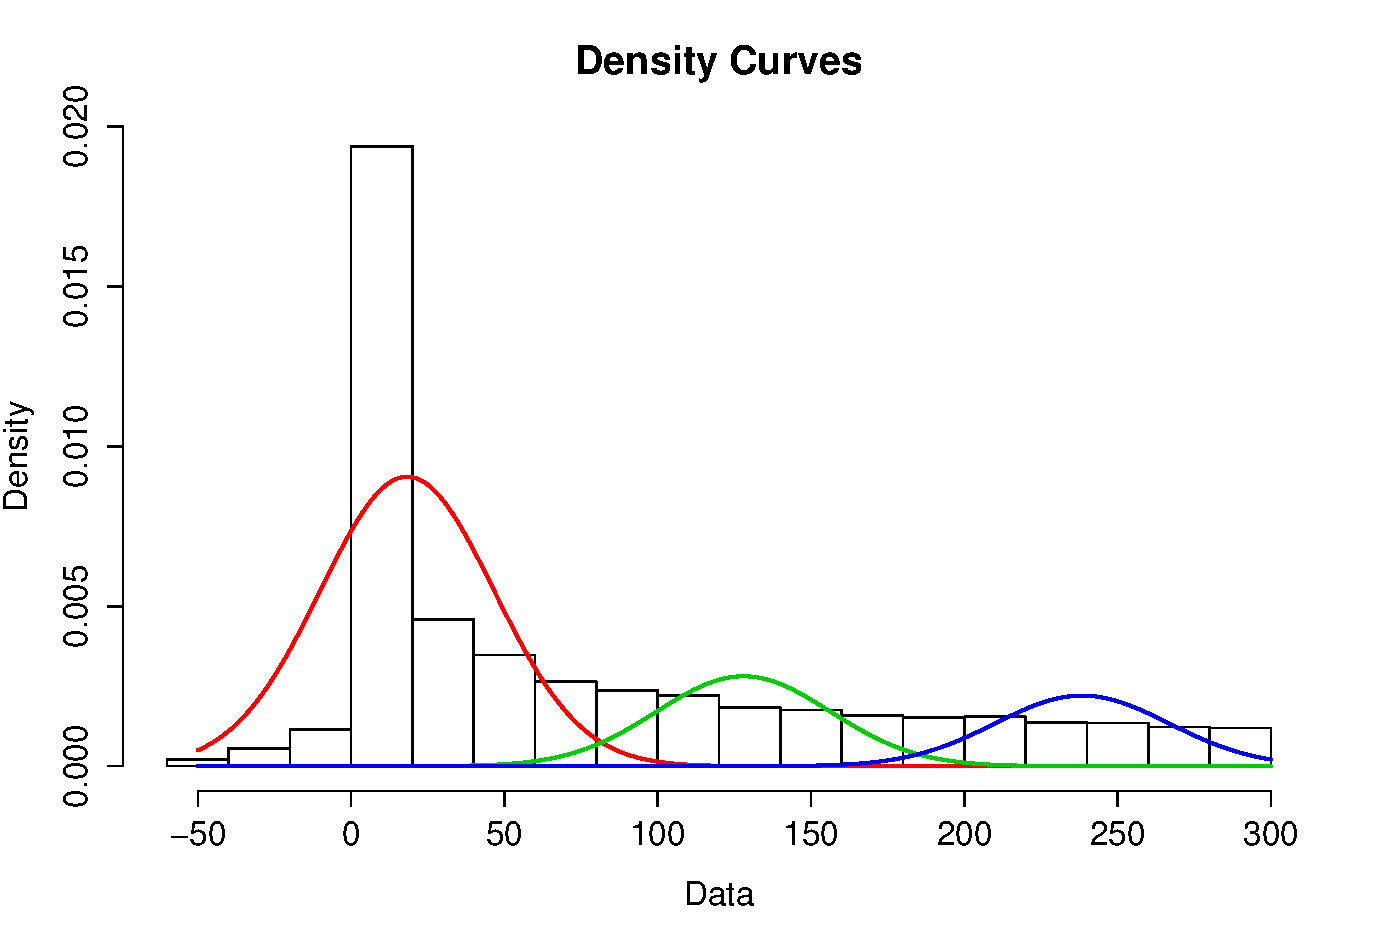
\includegraphics[width=70mm]{figures/CajaMarmixtureBalanceNonDef}\\
  \end{tabular}
    \caption{\label{Figure:cajamarMixt}Mixture of Gaussian approximation of \textit{end-of-day balance} for defaulter (left) and non-defaulter (right).}
\end{figure}

\textcolor{red}{Check please!}There exist however discrete (non-ordinal) predictive attributes which impose a limitation in the structure of the Conditional Gaussian network, since discrete attributes cannot have continuous parents. This might not be a problem for the semi-naive Bayesian network to be considered, and it is certainly not a problem for naive Bayes. Nonetheless, if this limitation were found to be problematic in future stages of the project then other families of probability distributions will be explored, such as Mixture of Truncated Exponentials[] or Mixture of Truncated Basis Functions[], which can cope with more generic Bayesian structures at a higher computation cost. 

In summary and given the original relational database, the process of building this static model consists of the following steps:\textcolor{blue}{(Should this be included?)}.

\begin{itemize}
\item Construct a single flat table, containing information on time windows of \emph{180 days}.
\item Build a semi-naive BN classifier (e.g NB or TAN). 
\item Update risk profiles using the static classifier.
\end{itemize}


%\begin{figure}[ht]
%\begin{center}
%\begin{tikzpicture}[->,>=stealth,shorten >=1pt,auto,node distance=2cm,semithick,
%        amarillo/.style={fill=yellow,rectangle,draw},
%        rojo/.style={fill=red,rectangle,draw,rounded corners}]
%        \node[green] (default) {Default};
%        \node (dot) [below of=default] {$\cdots$};
%        \node[amarillo] (tran1) [left of=dot] {Day -180};
%        \node[amarillo] (tran180) [right of=dot] {Day -1};
%        \draw (default) to (tran1);
%        \draw (default) to (tran180);
%\end{tikzpicture}
%\end{center}
%\caption{\label{Figure:CajaMarStatic}Global structure of the static model. Each yellow box represents a set of variables measures during the same day.
%The variables within a box can be connected (according to a tree structure and, globally, conforming a TAN).}
%\label{fig:static}
%\end{figure}
%---------------------------------------------------------------------------------------------



%\begin{figure}[ht]
%\begin{center}
%\begin{tikzpicture}[->,>=stealth,shorten >=1pt,auto,node distance=3cm,semithick,
%        amarillo/.style={fill=yellow,rectangle,draw},
%        rojo/.style={fill=red,rectangle,draw,rounded corners}]
%        \node[rojo] (default1) {Default -180};
%        \node[amarillo] (tran1) [below of=default1] {Day -180};
%        \node[rojo] (default2) [right of=default1] {Default -179};
%        \node[amarillo] (tran2) [below of=default2] {Day -179};
%        \node (dot) [right of=tran2] {$\cdots$};
%        \node (blank) [above of=dot] {$~~$};
%        \node[amarillo] (tran180) [right of=dot] {Day -1};
%        \node[rojo] (default180) [above of=tran180] {Default -1};
%        \draw (default1) to (tran1);
%        \draw (default2) to (tran2);
%        \draw (default180) to (tran180);
%        \draw (default1) to [bend left=45] (default2);
%        \draw (default2) to [bend left=45] (blank);
%        \draw (blank) to [bend left=45] (default180);
%        \draw (tran1) to [bend right=45] (tran2);
%        \draw (tran2) to [bend right=45] (dot);
%        \draw (dot) to [bend right=45] (tran180);
%\end{tikzpicture}
%\end{center}
%\caption{Global structure of the dynamic model. Each yellow box represents a set of variables measures during the same day.
%The variables within a box can be connected (according to a tree structure and, globally, conforming a TAN) as well as variables between two consecutive days. Red box refer to the possibility that 
%client is defaulter and are temporal connected.}
%\label{fig:global_temp}
%\end{figure}
%---------------------------------------------------------------------------------------------


%---------------------------------------------------------------------------------------------
\subsubsection*{Dynamic Model} 

In this second approach, we will consider the dynamic structure of the problem. These dynamics are present because the behaviour of the customers evolves over time (e.g. the account balance is continuously changing from one month to another, also the income levels, etc.)  as well as the label as a defaulter or non-defaulter customer (e.g. customers can be creditworthy and, after some time, go bankrupt because they have lost their job). \textcolor{blue}{Analysing some of the data, we can actually see that if a customer was a defaulter at day $t$, the probability of being a defaulter at day $t+1$ changes from $p$ (prior probability in the static model) to $p'$ (transition probability in the dynamic model). The reason for this dramatic change is that once a client is a defaulter, he/she will be a defaulter for some time, and the static model is unable to represent this effect.} \textcolor{red}{ And the way we have defined the problem it actually does not matter much, does it?} 




%\begin{figure}[ht]
%\begin{center}
%\begin{tikzpicture}
%  \node[circle,fill=yellow,draw, minimum size=1.1cm] (Xt1) at (1,1) {$X_{t-1}$};
%  \node[circle,fill=yellow,draw, minimum size=1.1cm] (Xt) at (5,1) {$X_t$};
%  \node[circle,fill=green,draw, minimum size=1.1cm] (avg) at (3,3) {$\bar{X}_t$};
%  \node[circle,fill=cyan,draw, minimum size=1.1cm] (ind) at (3,-2) {$\delta_{X_t}$};
%  \node[circle,fill=red,draw, minimum size=1.1cm] (D) at (5,5) {$D_t$};
%  \node[circle,fill=red,draw, minimum size=1.1cm] (Dt1) at (1,5) {$D_{t-1}$};
%  
%  \node at (0,3) {$\cdots$};
%  \node at (6,3) {$\cdots$};
%  
%  \draw[->] (Dt1) to (Xt1);
%  \draw[->] (Dt1) to (D);
%  \draw[->] (D) to (Xt);
%  \draw[->] (D) to (avg);
%  \draw[->] (Xt1) to (Xt);
%  \draw[->] (avg) to (Xt);
%  \draw[->] (ind) to (Xt);
%  
%  
%  
%\end{tikzpicture}
%\end{center}
%\caption{Basic component of the structure of the dynamic model.}
%\label{fig:component}
%\end{figure}

\begin{figure}
\begin{center}
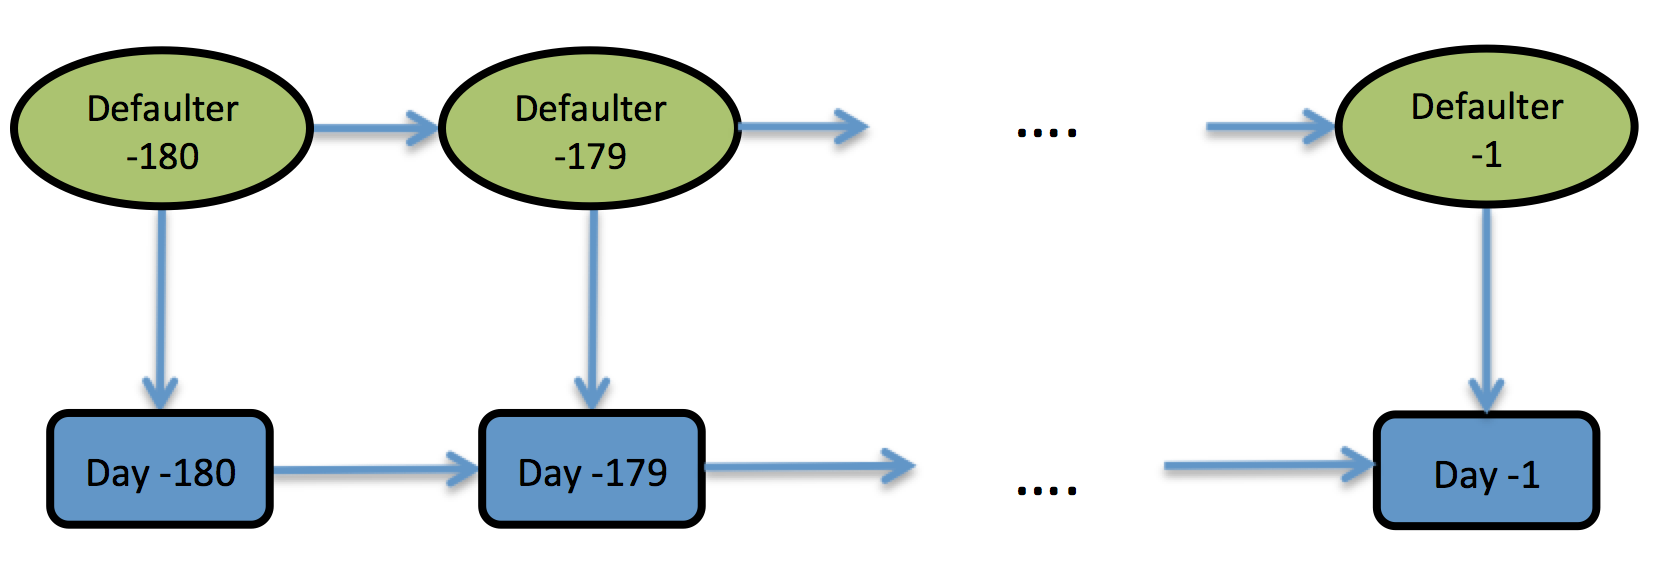
\includegraphics[scale=0.45]{./figures/CajaMarModel1}
\caption{Global structure of the dynamic model. Each yellow box represents a set of variables measures during the same day.
The variables within a box can be connected (according to a tree structure and, globally, conforming a TAN) as well as variables between two consecutive days. Red box refer to the possibility that 
client is defaulter and are temporal connected.}
\label{fig:global_temp}
\end{center}
\end{figure}

\begin{figure}
\begin{center}
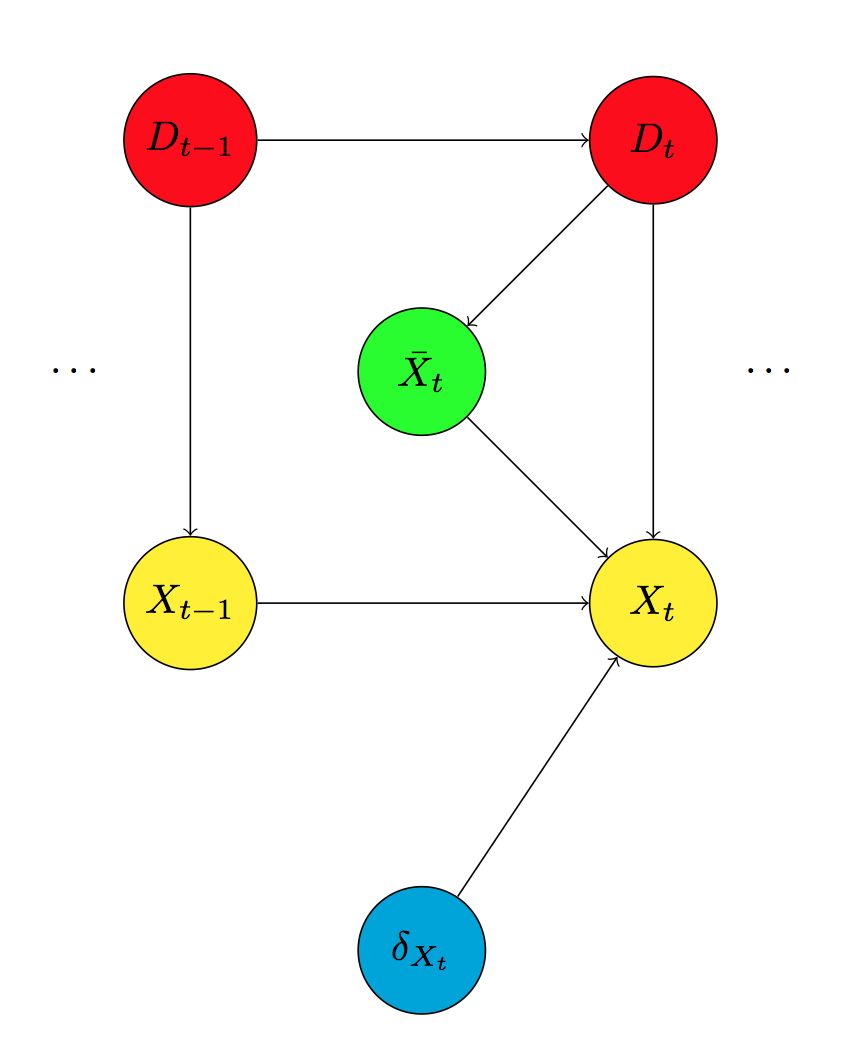
\includegraphics[scale=0.45]{./figures/CajaMarModel2}
\caption{Basic component of the structure of the dynamic model.}
\label{fig:component}
\end{center}
\end{figure}


Figure~\ref{fig:global_temp} represents the global idea of the proposed temporal model. It can be compactly represented by a dynamic Bayesian network made of components as the one displayed in 
Figure~\ref{fig:component}. $D_t$ represents the class variable at time slice $t$ (i.e. defaulting or non-defaulting client). Each feature variable at time $t$, denoted as $X_t$, is linked to the same variable at time $t+1$, $X_{t+1}$. Although this is a reasonable assumption for most of the variables, this first Markov order relationship however might prove insufficient for some of the variables.\textcolor{red}{[We include the following comments to justify the introduction of memory variables. We think that we need to introduce memory variables if we have evidence that first order Markov relationships does not hold and we need to account for information coming from the past. This evidence could be obtained for a partial corrrelogram.]}. \textcolor{red}{Figures \ref{fig:cajamarPC1order} and FigY (FigY should show a couple of partial correlograms that do not drop to zero at lag $2$)  show the partial correlograms for different continuous predictive variables. For the variables in Figure \ref{fig:cajamarPC1order}, the partial correlograms drop to almost zero for a lag equal to $2$, making the first Markov order assumption a reasonable one. However, for the variables in Figure FigY the partial correllogram takes more time to drop to zero, which might indicate that past samples still have an influence on the current sample given the previous one.} To mitigate this effect,  a \emph{memory variable}, $\bar{X}_t$, that represents the average value of $X$ during the last $180$ time slices (days) is included. 


\begin{figure}
  \centering
    \begin{tabular}{cc}
    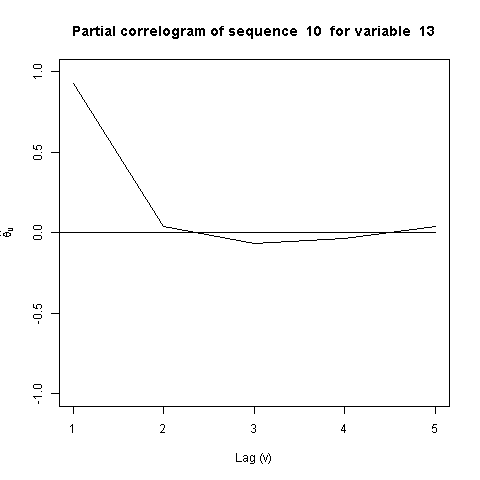
\includegraphics[width=70mm]{figures/CajaMarpcrl13}&
    \begin{minipage}[b]{0.45\linewidth} Partial correllogram for another variable\end{minipage}\\
  \end{tabular}
    \caption{\label{fig:cajamarPC1order}Partial correllogram for variables A and B. A first order Markov assumption seems reasonable.}
\end{figure}


Finally, an indicator variable $\delta_{X_t}$ may be included if the variable is such that is observed many times at point 0. This is the case for payments made by credit card or the historical monthly outstanding amount on the account for instance, whose value can be equal to zero for a large number of days for most customers, as shown in Figure \ref{fig:CajamarIndicatorVar}. Figure \ref{fig:CajamarIndicatorVar}(a) displays the histogram of this variable including all values, and \ref{fig:CajamarIndicatorVar}(b) when the zero values are not considered.

\begin{figure}
  \centering
    \begin{tabular}{cc}
    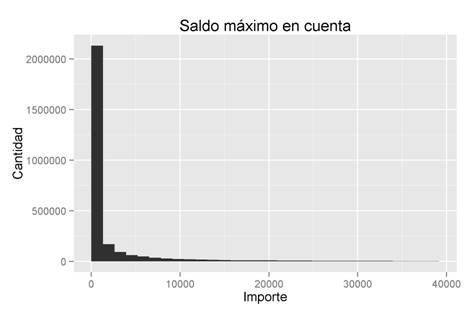
\includegraphics[width=70mm]{figures/CajaMarOutsAmount}&
    \begin{minipage}[b]{0.45\linewidth} Outstanding amount without zeros\end{minipage}\\
  \end{tabular}
    \caption{\label{fig:CajamarIndicatorVar}Frequency histogram of the historical monthly outstanding amount}
\end{figure}

On the other hand, there exist some variables that do not display any type of dynamic behaviour. This is for instance the case for variables \textcolor{red}{1 and 3 (please replace with the names of the vars.)}, whose correllograms on Figure \ref{fig:cajamarCorr} show values very close to zero for all lags. These variables are hence not linked through consecutive time steps, which are represented by $Y_{t}$ and $Y_{t+1}$ in Figure \ref{fig:component}. \textcolor{red}{What about drawing only one $Y$? aren't we including the socio-economic variables pointing at the class variable?}. 

\begin{figure}
  \centering
    \begin{tabular}{cc}
    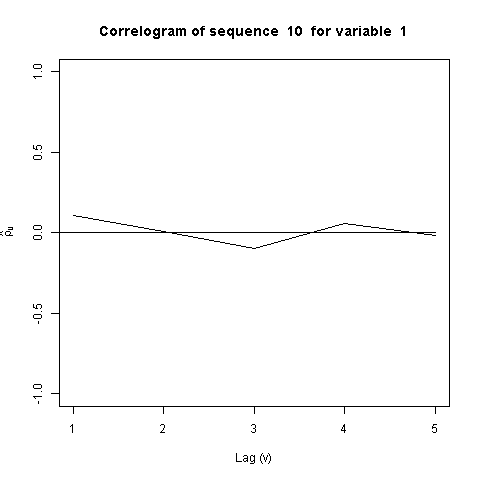
\includegraphics[width=70mm]{figures/CajaMarcrl1}&
     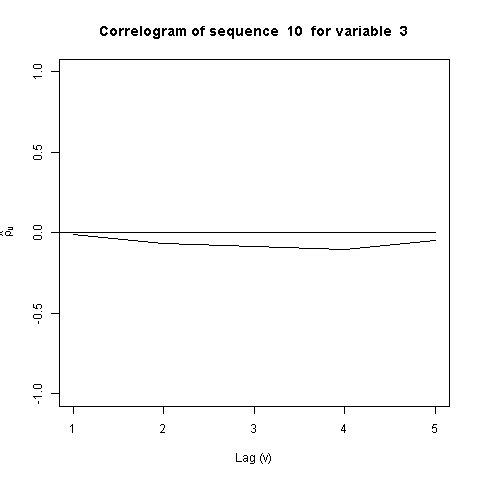
\includegraphics[width=70mm]{figures/CajaMarcrl3}\\
  \end{tabular}
    \caption{\label{fig:cajamarCorr}Correllogram for variables 1 and 3. No temporal dynamic shown.}
\end{figure}


In summary, the process of building this dynamic model from the original relational database consists of the following steps:\textcolor{blue}{(Should this be included?)}.

\begin{itemize}
\item Construct \emph{1 flat table} for each day.
\item Build a \emph{dynamic} BN classifier (e.g. NB or TAN like structure extended in a dynamic fashion). 
\item Update risk profiles using the dynamic classifier.
\end{itemize}

%%%%%%%%%%%%%%%%%%%%%%%%%%%%%%%%%%%%
\subsubsection{Low risk profile extraction}
%%%%%%%%%%%%%%%%%%%%%%%%%%%%%%%%%%%%
\subsubsection*{Introduction of the problem}

The marketing department at Cajamar periodically launches marketing campaigns for the recruitment of new products by customers (i.e. a new credit card, an insurance, ...). The success of these campaigns depends greatly on the client group to which the campaign has finally targeted. It is also crucial to reduce as much as possible unnecessary expenses focused on non-potential customers. 

For this purpose, the marketing group proceeds as follows. First, they filter the customers using their own marketing models and also, in collaboration with the risk department, select a subset of predictors considered relevant to be part of the final profile (mainly sociodemographic variables). For example, the age of a client is a relevant predictor when designing campaigns to attract customers for a death insurance. 

After obtaining this first group of customers for the campaign and determining the set of relevant attributes, the model proposed in Section~\ref{SubSection:Predicting} will be used to identify the profiles of the less risky clients using the most probable explanations (MPE) method (\emph{defaulter} variable is evidenced to \emph{No}) . Thus, the target customers previously filtered can be now grouped and ranked using these profiles.


\subsubsection*{Static model}

As pointed out before, mainly sociodemographic variables will determine the customer profiles used in the campaigns. These variables are mostly static as they do not change frequently over time (e.g. marital status, sex, type of job, ...). Hence, it has more sense to explore a profile extraction solution based on a static model as the one depicted in Fig.~\ref{fig:StaticBNProfile}. A solution could be the use of augmented Bayesian classifiers like TAN, $k$-DB to reduce the search space required for general structures. 


\begin{figure}[h]
\centering
\begin{tikzpicture}[->,>=stealth,shorten >=1pt,auto,node distance=2cm,semithick,
        azul/.style={fill=cyan,rectangle,draw},
        verde/.style={fill=green,ellipse,draw}]
        \node[verde] (default) {Default};
        \node[azul] (predictors) [below of=default] {Predictors};
        \draw (default) to (predictors);
\end{tikzpicture}
\caption{Static Bayesian network for the profile extraction. The variables within the blue box can be connected to conform an augmented Bayesian classifier.}
\label{fig:StaticBNProfile}
\end{figure}


%---------------------------------------------------------------------------------------------


Note that past information about the variables are not considered for this problem as it was for predicting the probability of defaulting in Section~\ref{SubSection:Predicting}. In this model the latest information about the variables are considered instead.

For the profile extraction, the model not necessarily must have a classifier structure but it can have a general structure instead. However, what is desirable is to avoid using a NB structure for this task. The reason is that once the \emph{defaulter} variable is evidenced to \emph{No}, the predictors become independent and the analysis would be poorer (MPE in this case would correspond to the maximum probability value for each variable individually).



\subsubsection*{Dynamic model}

A dynamic model for the profile extraction makes no sense as the variables used are mainly sociodemographic and their values do not change over time.

\textcolor{blue}{We could include some plots showing that sociodemographic variables does not change over time?}

%\subsubsection*{Model Structure}
%
%From a probabilistic modelling point of view, Caja-Mar faces two different problems [][]: the prediction of the risk of defaulting of a customer in the next two years; and the extraction of profiles of ``desirable'' prospective customers. 
%
%The risk prediction problem has been modelled as supervised dynamic prediction problem.  We are given a data base with a set of variables or predictors (some of them manually built by CajaMar's experts) describing the financial behaviour of the customers and, also, whether the customer is considered as defaulter and non defaulter according to CajaMar standards (i.e. a binary class variable). The dynamic component of the problem needs to be considered because the behaviour of the customers evolves over time (e.g. the account balance is continuously changing from month to another, the level of incomes, etc.)  as well as the labelling as defaulter or non-defaulter customer (e.g. one customer can be creditworthy and, but after some time, be in bankrupt for becoming unemployed). More specifically, the proposed model is expected to answer the following question: which is the probability that this customer will  default in some of his/her loans in two years? And this prediction has to be made only using the customer's behavior in the last 180 days \footnote{This limit is imposed by the Bank of Spain.}.
%
%The graphical structure of the dynamic probabilistic graphical model devised for this problem is given in Figure \ref{Figure:CajaMarModel1}.  The yellow square boxes ``Day -180'', ..., ``Day-1'' represents the temporal evolution of the predictor variables. The model only refers to 180 days because this is the imposed limit of days when making predictions. Similarly, the class variable ``default'' is assumed to evolve over time but with the relevant different that the default class sequence refers to a point in the time \textbf{two years later} than  the point in the time the daily predictor variables. 




